\documentclass[aspectratio=169, 11pt]{beamer}

% ====== Theme ======
\usetheme{Madrid}
\definecolor{CityUBlue}{RGB}{0, 51, 102}
\definecolor{CityULightBlue}{RGB}{0, 102, 179}
\definecolor{CityUGold}{RGB}{198, 163, 0}
\usecolortheme[named=CityUBlue]{structure}
\setbeamercolor{title}{fg=white, bg=CityUBlue}
\setbeamercolor{frametitle}{fg=white, bg=CityUBlue}
\setbeamercolor{block title}{bg=CityUBlue, fg=white}
\setbeamercolor{block body}{bg=CityUBlue!10, fg=black}
\setbeamercolor{item}{fg=CityUBlue}
\setbeamercolor{subitem}{fg=CityULightBlue}

% ====== Packages ======
\usepackage[T1]{fontenc}
\usepackage{lmodern}
\usepackage{booktabs}
\usepackage{graphicx}
\usepackage{hyperref}
\usepackage{amsmath, amssymb}
\usepackage{tikz}
\usepackage{appendixnumberbeamer}

% ====== Settings ======
\setbeamertemplate{navigation symbols}{}
\graphicspath{{figures/}{../../Figures used in slides/}}

% ====== Metadata ======
\title[EF8083 Lecture 4]{PhD Lecture in Behavioral Asset Pricing:\\ Preferences \& Beliefs (II)}
\author[F.\ W.\ Li]{Frank Weikai Li}
\institute[CityU]{Associate Professor of Finance\\City University of Hong Kong}
\date{}

% ==============================================================================
\begin{document}
% ==============================================================================

% --- Slide 1: Title ---
\begin{frame}[plain]
\titlepage
\end{frame}

% --- Slide 2: Section ---
\section{Psychology of Beliefs}

\begin{frame}{}
\vfill
\centering
{\Large \textbf{Psychology of Beliefs}}
\vfill
\end{frame}

% --- Slide 3: Representativeness ---
\begin{frame}{Psychology of Beliefs: Representativeness}
\begin{itemize}
\item Consider questions such as:
  \begin{itemize}
  \item What is the probability that object A comes from class B?
  \item What is the probability that event A was generated from process B?
  \end{itemize}
\item Kahneman and Tversky (1974) argue that people often answer by using the ``representativeness heuristic''
  \begin{itemize}
  \item Evaluate the probability by the extent to which A is representative of B
  \item i.e.\ degree to which A reflects the essential characteristics of B
  \end{itemize}
\item This is helpful in general but can lead to serious biases
\end{itemize}
\end{frame}

% --- Slide 4: Base-rate neglect ---
\begin{frame}{Representativeness, ctd.}
\begin{itemize}
\item \textbf{Base-rate neglect}
\item Consider the following description:
  \begin{itemize}
  \item Steve is very shy and withdrawn, invariably helpful, but with little interest in people or in the world of reality. A meek and tidy soul, he has a need for order and structure, and a passion for detail.
  \end{itemize}
\item People judge Steve to be more likely a librarian than a farmer
\item But there are 20 times more farmers than librarians in the U.S.
\end{itemize}
\vfill
\centering
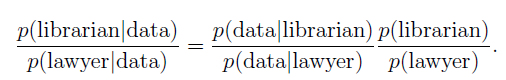
\includegraphics[width=0.35\textwidth]{figures/slide04_pic4.png}
\end{frame}

% --- Slide 5: Sample size neglect ---
\begin{frame}{Representativeness, ctd.}
\begin{itemize}
\item \textbf{Sample size neglect, ctd.}
\item When we do not know the model generating the data, we may infer it too quickly based on too little data
\item This can lead to over-extrapolation of recent trends
\item E.g., the hot hand fallacy
  \begin{itemize}
  \item Seeing a basketball player make a few shots in a row leads to the belief that he is ``hot''
  \item But empirical evidence suggests that the hot hand is largely a myth (Gilovich, Vallone, and Tversky, 1985)
  \end{itemize}
\end{itemize}
\end{frame}

% --- Slide 6: Overconfidence ---
\begin{frame}{Psychology of Beliefs: Overconfidence}
\begin{itemize}
\item At least two distinct types:
\item \textbf{Overprecision}
  \begin{itemize}
  \item People are too confident in the accuracy of their forecasts
  \item 98\% confidence intervals include the true quantity around 60\% of the time (Alpert and Raiffa, 1982)
  \end{itemize}
\item \textbf{Overplacement}
  \begin{itemize}
  \item People think they are better than others
  \item 90\% of drivers think they are above-average drivers (Svenson, 1981)
  \end{itemize}
\end{itemize}
\end{frame}

% --- Slide 7: Overprecision Survey Evidence ---
\begin{frame}[shrink=5]{Overprecision: Survey Evidence}
\begin{itemize}
\item Ben-David, Graham and Harvey (2013)
\item CFO's expected stock market return distribution is too narrow
\item Realized market returns are within the executives' 80\% confidence intervals only 36\% of the time
\end{itemize}
\vfill
\centering

\includegraphics[width=0.55\textwidth]{figures/slide07_pic4.jpg}
\end{frame}

% --- Slide 8: Excessive Trading ---
\begin{frame}[shrink=5]{Overconfidence: Excessive Trading}
\begin{itemize}
\item \textbf{Excessive trading}
  \begin{itemize}
  \item Under efficient markets, no trading other than liquidity needs and portfolio rebalancing
  \item Speculative trading reflects differences of opinion and some amount of overconfidence
  \end{itemize}
\item Trading leads to lower returns
  \begin{itemize}
  \item The more you trade, the lower your return (Odean, 1999)
  \end{itemize}
\end{itemize}
\vfill
\centering
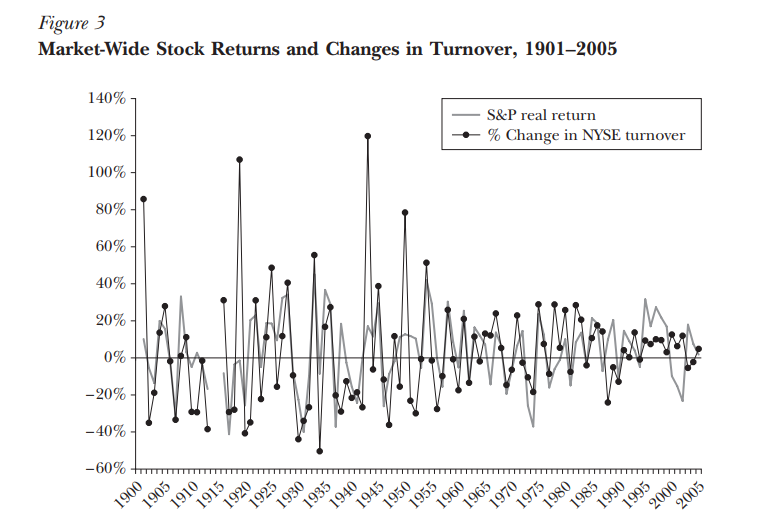
\includegraphics[width=0.55\textwidth]{figures/slide08_pic6.png}\\[0.2em]
\footnotesize Hong and Stein (2007)
\end{frame}

% --- Slide 9: Boys will be boys ---
\begin{frame}[shrink=5]{Overconfidence: Excessive Trading}
\begin{itemize}
\item \textbf{Boys will be boys}
\item Barber and Odean (2001) show that men trade more frequently than women, but earn lower return
\item Consistent with psychological studies that men are more overconfident than women (Lundeberg et al., 1994)
\end{itemize}
\vfill
\centering
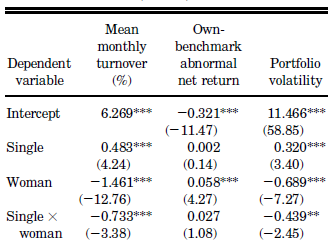
\includegraphics[width=0.42\textwidth]{figures/slide09_pic3.png}
\hspace{0.3em}

\includegraphics[width=0.42\textwidth]{figures/slide09_pic4.png}
\end{frame}

% --- Slide 10: Momentum and Overconfidence ---
\begin{frame}{Overconfidence: Momentum}
\begin{itemize}
\item Daniel, Hirshleifer, and Subrahmanyam (1998)
\item Momentum is driven by investor overconfidence and self-attribution bias
  \begin{itemize}
  \item Investors are overconfident in the private information they gather
  \item Investors also suffer from self-attribution bias: they credit themselves for successes but blame external factors for failures
  \end{itemize}
\item Positive returns reinforce overconfidence, leading to more aggressive trading and price momentum
\item Eventually, prices correct when information is revealed
\end{itemize}
\end{frame}

% --- Slide 11: Momentum and Individualism ---
\begin{frame}{Overconfidence: Momentum}
\begin{itemize}
\item Chui, Titman, and Wei (JF 2010) test the idea that momentum is driven by investor overconfidence and self-attribution bias
\item They use an individualism index developed by Hofstede (2001) to proxy for investor overconfidence
\item They find that momentum is stronger in countries with higher individualism scores
\end{itemize}
\vfill
\centering
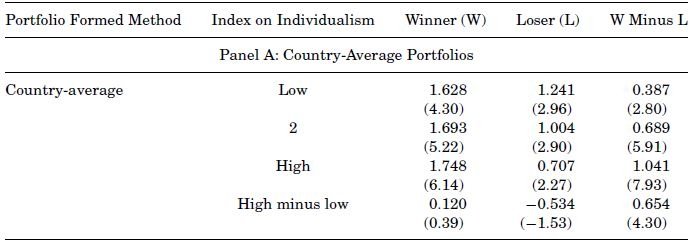
\includegraphics[width=0.55\textwidth]{figures/slide11_pic4.jpg}
\end{frame}

% --- Slide 12: Over-extrapolation ---
\begin{frame}{Psychology of Beliefs: Over-extrapolation}
\begin{itemize}
\item Estimate of the future value of a quantity is a positive function of the recent past values of that quantity
\item Most important and widely-applied ideas in the behavioral finance
\item The source of over-extrapolation: representativeness heuristic
\item Application to finance:
  \begin{itemize}
  \item Return extrapolation: predict future returns based on past returns
  \item Fundamentals extrapolation: predict future earnings/cash flows based on past growth
  \end{itemize}
\end{itemize}
\end{frame}

% --- Slide 13: Over-extrapolation conceptual framework ---
\begin{frame}{Over-extrapolation: Conceptual Framework}
\vfill
\centering
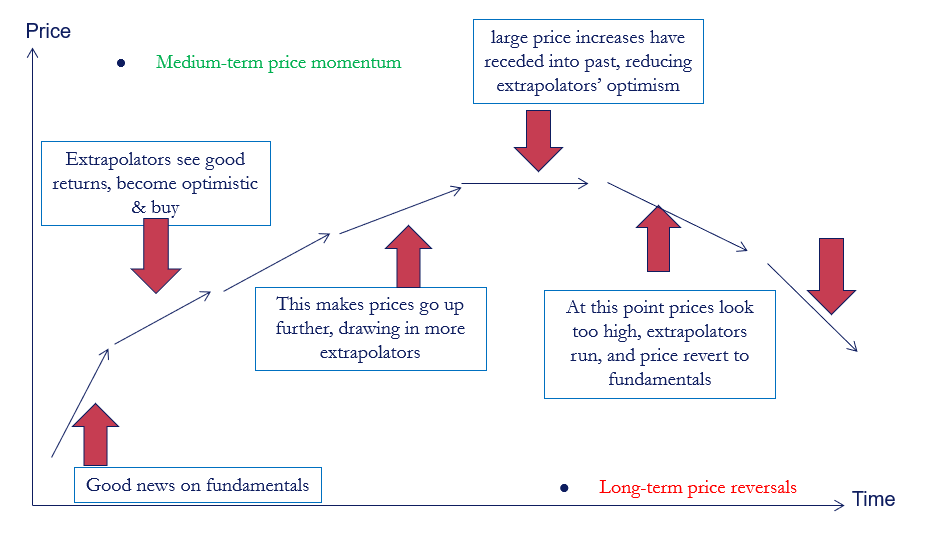
\includegraphics[width=0.65\textwidth]{figures/13.png}\\[0.2em]
\end{frame}

% --- Slide 14: Survey Evidence ---
\begin{frame}{Over-extrapolation: Survey Evidence}
\begin{itemize}
\item \textbf{Excess volatility and predictability in aggregate stock market}
\item Extrapolators buy assets whose prices have risen because they expect them to keep rising
\item This leads to overvaluation and return predictability
\end{itemize}
\vfill
\centering
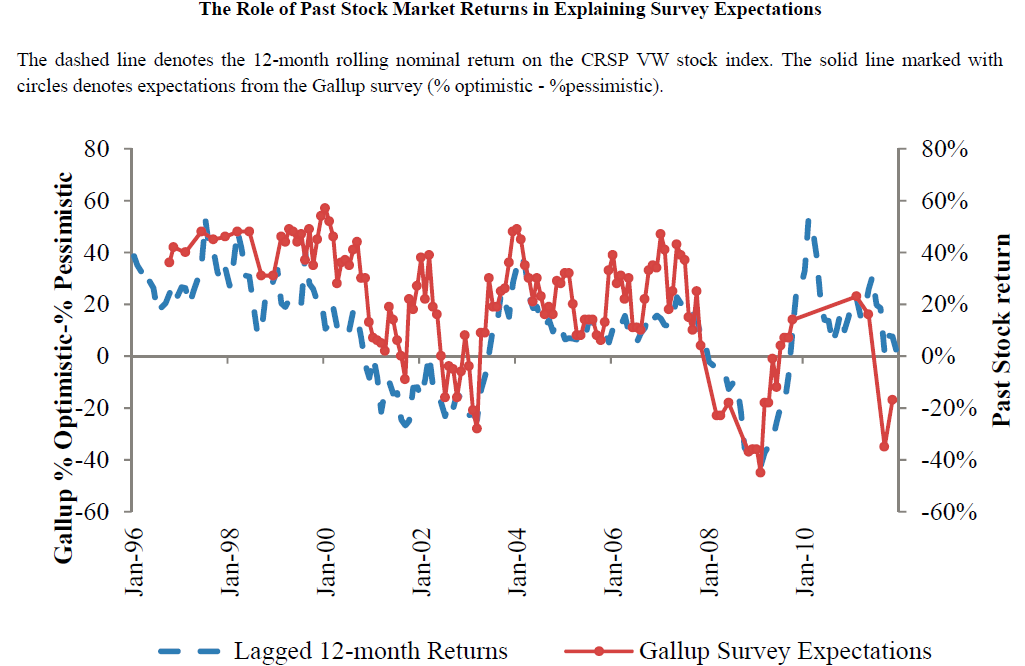
\includegraphics[width=0.55\textwidth]{figures/slide14_pic4.png}\\[0.2em]
\footnotesize Greenwood and Shleifer (2014)
\end{frame}

% --- Slide 15: Survey Evidence ctd ---
\begin{frame}[shrink=5]{Over-extrapolation: Survey Evidence}
\begin{itemize}
\item Investors act on their over-extrapolative beliefs with flows into (out of) stock markets
\end{itemize}
\vfill
\centering
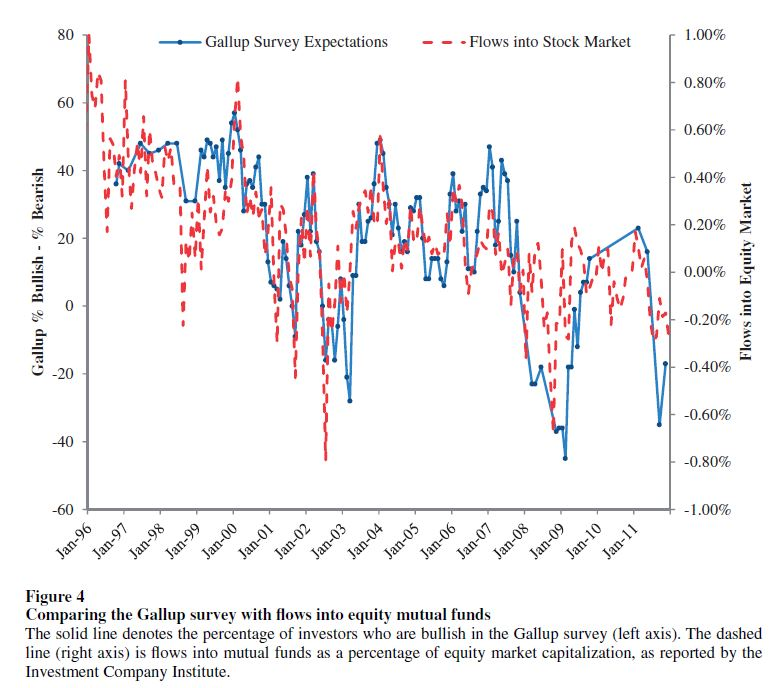
\includegraphics[width=0.55\textwidth]{figures/slide15_pic4.jpg}\\[0.2em]
\footnotesize Greenwood and Shleifer (2014)
\end{frame}

% --- Slide 16: DOX ---
\begin{frame}[shrink=10]{Over-extrapolation of Past Returns: Applications}
\begin{itemize}
\item Using survey data on expectations of stock returns, Cassella and Gulen (RFS 2018) estimate the degree of extrapolative thinking in investors' beliefs (DOX) about market return
\item DOX ($1-\lambda$) measures the weight investors place on past returns
\end{itemize}
\vfill
\centering

\includegraphics[width=0.42\textwidth]{figures/slide16_pic4.png}
\hspace{0.3em}
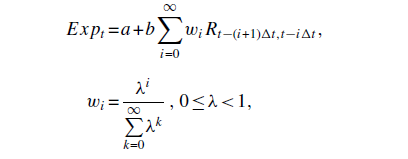
\includegraphics[width=0.42\textwidth]{figures/slide16_pic5.png}\\[0.2em]
\footnotesize A lower $\lambda$ implies that investors place higher weight on more recent observations, while earlier observations contribute less to an extrapolator's expectations
\end{frame}

% --- Slide 17: DOX and Predictability ---
\begin{frame}[shrink=5]{Over-extrapolation of Past Returns: Applications}
\begin{itemize}
\item They find the predictability of stock returns by price-scaled variable (e.g., D/P, B/M or E/P) is contingent on the DOX
\item When DOX is high, investors more quickly ``forget'' the positive price changes that drove up valuations, making them less prone to extrapolate recent returns
\item As a result, high valuations are more informative about low future returns when DOX is high
\end{itemize}
\vfill
\centering
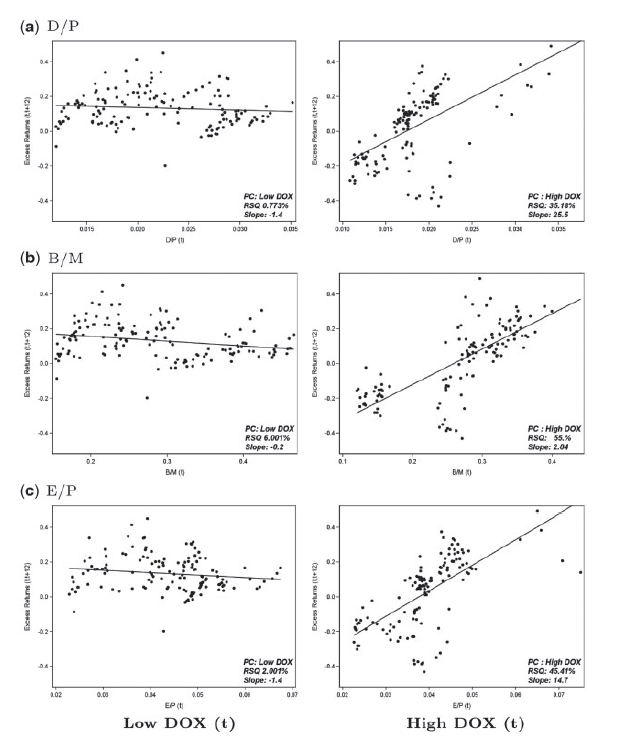
\includegraphics[width=0.55\textwidth]{figures/slide17_pic4.png}
\end{frame}

% --- Slide 18: Fundamentals Extrapolation ---
\begin{frame}{Over-extrapolation of Past Fundamentals: Application}
\begin{columns}[T]
\begin{column}{0.50\textwidth}
\begin{itemize}
\item Bordalo et al.\ (2023): overreaction of long-term earnings growth (LTG) expectation help explain time-series variation in P/D ratio and predict aggregate market return
\item Good news cause investors to become overly optimistic about future earnings growth
\end{itemize}
\end{column}
\begin{column}{0.48\textwidth}
\centering
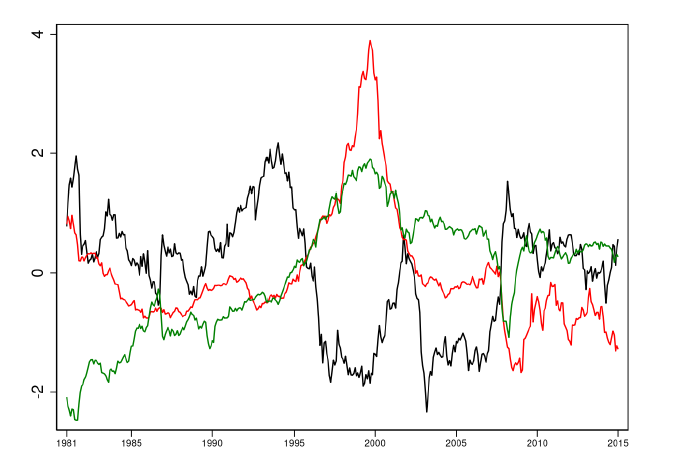
\includegraphics[width=\textwidth]{figures/slide18_pic3.png}\\[0.2em]
\footnotesize This figure graphs LTG (red) and the price dividend ratio (green) together with realized stock returns in the coming five years (black)\\[0.2em]
Bordalo et al.\ (2023)
\end{column}
\end{columns}
\end{frame}

% --- Slide 19: Conservatism ---
\begin{frame}{Psychology of Beliefs: Conservatism}
\begin{itemize}
\item Investors with extrapolative or overconfident beliefs adjust their views too much in response to new information and cause excessive movements in prices
\item But some phenomena --- momentum and PEAD --- may instead require that investors adjust their views \emph{too little}
\item \textbf{Conservatism}: Individuals are too slow to update their beliefs in response to new information (Edwards, 1968)
\end{itemize}
\end{frame}

% --- Slide 20: Belief Perseverance ---
\begin{frame}{Psychology of Beliefs: Belief Perseverance and Confirmation Bias}
\begin{itemize}
\item \textbf{Belief perseverance:}
  \begin{itemize}
  \item Once we have formed an opinion, we are often too slow to change it on receipt of new evidence
  \item We don't look for evidence that would falsify our beliefs
  \item We ignore evidence that goes against our beliefs
  \end{itemize}
\item \textbf{Confirmation bias:}
  \begin{itemize}
  \item We actively seek out evidence that supports our beliefs
  \item We interpret ambiguous evidence as supportive of our beliefs
  \end{itemize}
\end{itemize}
\end{frame}

% --- Slide 21: Anchoring ---
\begin{frame}{Psychology of Beliefs: Anchoring}
\begin{itemize}
\item Kahneman and Tversky (1974): in forming numerical estimates of uncertain quantities, adjustments in assessments away from some initial value (called the ``anchor'') are often insufficient
\item E.g.\ estimates of the percentage of African countries in the UN are affected by a random number generated by spinning a wheel
\item Anchoring effects persist even when the anchor is clearly irrelevant
\item Applications in finance: IPO pricing, analyst forecasts, merger valuations
\end{itemize}
\end{frame}

% --- Slide 22: Effect of Feelings ---
\begin{frame}{The Effect of Feelings}
\begin{itemize}
\item A recent strand of research investigates how feelings affect beliefs and preferences
  \begin{itemize}
  \item Affective feelings (mood, emotion)
  \item Cognitive feelings
  \end{itemize}
\item \textbf{Affective feelings}
  \begin{itemize}
  \item A happier mood caused by an exogenous stimulus leads to more optimistic judgments and choices
  \item A sadder mood leads to more pessimistic judgments
  \item E.g.\ sunshine, sports outcomes, holidays
  \end{itemize}
\end{itemize}
\end{frame}

% --- Slide 23: Affective Feelings - Sports ---
\begin{frame}{Affective Feelings: Applications}
\begin{itemize}
\item \textbf{Sports}
\item Edmans, Garcia, and Noli (2006): When the national soccer team loses a World Cup match, the national stock market falls the next day
\item Disappointing sports news worsens the national mood, leading to lower stock returns
\item The effect is stronger in countries where soccer is more important
\end{itemize}
\end{frame}

% --- Slide 24: Affective Feelings - Terrorism ---
\begin{frame}{Affective Feelings: Applications}
\begin{itemize}
\item \textbf{Terrorist attacks}
\item Wang and Yang (2020): Terrorist attacks lead to increased aggregate risk aversion, as proxied by flows into (out of) government bond funds (equity funds)
\item These findings point to a mechanism by which feelings affect risk preferences
\end{itemize}
\end{frame}

% --- Slide 25: Cognitive Feelings ---
\begin{frame}{Cognitive Feelings}
\begin{itemize}
\item Feeling of ease when accessing or processing information leads to more positive judgements than justified by content alone (Zajonc, 1968; Bornstein, 1989)
\item E.g.\ people like familiar things more than justifiably
\item \textbf{Applications:}
  \begin{itemize}
  \item Home bias in portfolio choice
  \item Local bias in stock ownership
  \item Preference for stocks with pronounceable ticker symbols
  \end{itemize}
\end{itemize}
\end{frame}

% --- Slide 26: Section ---
\section{Heterogeneous Beliefs}

\begin{frame}{}
\vfill
\centering
{\Large \textbf{Heterogeneous Beliefs}}
\vfill
\end{frame}

% --- Slide 27: Overview ---
\begin{frame}{Heterogeneous Beliefs: Overview}
\begin{itemize}
\item Previously we look at the psychological foundations of systematically biased beliefs
  \begin{itemize}
  \item Assuming representative investor
  \end{itemize}
\item In this part, we look at models with heterogeneous beliefs
  \begin{itemize}
  \item Average belief is unbiased
  \item But cross-sectional variation in beliefs can still affect prices
  \end{itemize}
\end{itemize}
\end{frame}

% --- Slide 28: Heterogeneous Beliefs ctd ---
\begin{frame}{Heterogeneous Beliefs, ctd.}
\begin{itemize}
\item People regularly hold different beliefs about almost everything in life
  \begin{itemize}
  \item from political views and sport events to economic outcomes and asset returns
  \end{itemize}
\end{itemize}
\vfill
\centering

\includegraphics[width=0.55\textwidth]{figures/slide28_pic4.png}
\end{frame}

% --- Slide 29: Sources ---
\begin{frame}{Sources of Heterogeneous Beliefs}
\begin{itemize}
\item What may cause heterogeneous beliefs?
\item Asymmetric information alone cannot cause rational agents with common prior to agree to disagree
  \begin{itemize}
  \item e.g., No-trade Theorem of Milgrom and Stockey (1981)
  \end{itemize}
\item Heterogeneous beliefs must come from:
  \begin{itemize}
  \item Differences in prior beliefs
  \item Differences in how agents process information (bounded rationality)
  \item Overconfidence in private signals
  \end{itemize}
\end{itemize}
\end{frame}

% --- Slide 30: Experience Effects ---
\begin{frame}{Sources of Heterogeneous Beliefs --- Experience Effects}
\begin{columns}[T]
\begin{column}{0.50\textwidth}
\begin{itemize}
\item One important source of heterogeneous beliefs is personal experience
\item When forming beliefs, a rational individual should take account of all available information
\item However, mounting evidence suggests that people overweight their personal experience
\end{itemize}
\end{column}
\begin{column}{0.48\textwidth}
\centering
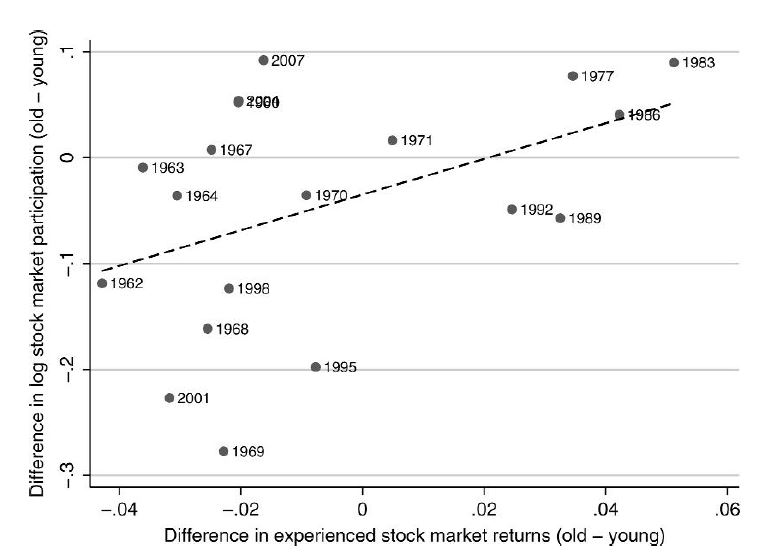
\includegraphics[width=\textwidth]{figures/slide30_pic3.jpg}
\end{column}
\end{columns}
\end{frame}

% --- Slide 31: Inflation Expectation ---
\begin{frame}{Sources of Heterogeneous Beliefs --- Experience Effects}
\begin{columns}[T]
\begin{column}{0.50\textwidth}
\begin{itemize}
\item \textbf{Inflation expectation} (Malmendier and Nagel, 2016)
\item Individuals overweight inflation experienced during their lifetimes when forming expectations about future inflation
\item Younger individuals update their beliefs more quickly
\item Older individuals place more weight on past inflation experiences
\end{itemize}
\end{column}
\begin{column}{0.48\textwidth}
\centering
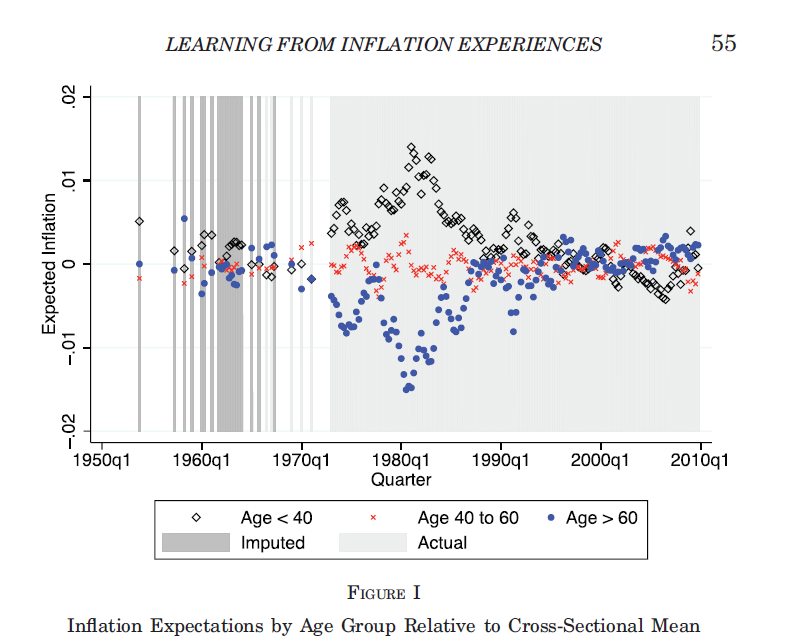
\includegraphics[width=\textwidth]{figures/slide31_pic3.png}\\[0.2em]
\footnotesize Malmendier and Nagel (2016)
\end{column}
\end{columns}
\end{frame}

% --- Slide 32: Political Polarization ---
\begin{frame}{Sources of Heterogeneous Beliefs --- Political Polarization}
\begin{columns}[T]
\begin{column}{0.50\textwidth}
\begin{itemize}
\item Goldman, Gupta and Israelsen (JFE 2025)
\item Setting: Comparing coverage of the same corporate financial news by the conservative Wall Street Journal and the liberal New York Times
\item \textbf{Findings:}
  \begin{itemize}
  \item Newspapers use more positive language for firms aligned with their political leanings
  \item Effect stronger for politically sensitive topics
  \end{itemize}
\end{itemize}
\end{column}
\begin{column}{0.48\textwidth}
\centering
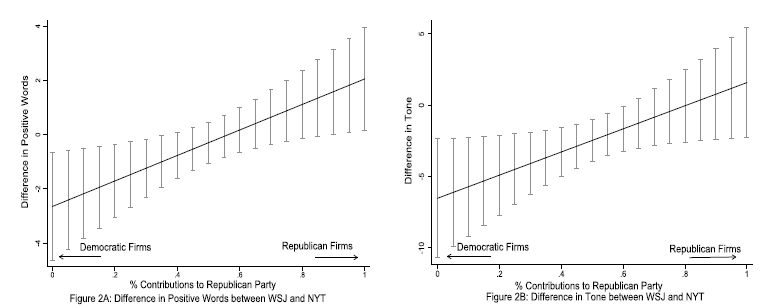
\includegraphics[width=\textwidth]{figures/slide32_pic4.png}
\end{column}
\end{columns}
\end{frame}

% --- Slide 33: No SSC ---
\begin{frame}{Heterogeneous Beliefs (no SSC)}
\begin{itemize}
\item Taken alone, overconfidence-based heterogeneous beliefs do not have interesting pricing effects
\item The pricing impacts of optimistic and pessimistic investors cancel out
\item But they can help explain the high trading volume
  \begin{itemize}
  \item Investors trade because they disagree about asset values
  \item Higher dispersion of beliefs $\Rightarrow$ higher trading volume
  \end{itemize}
\end{itemize}
\end{frame}

% --- Slide 34: With SSC ---
\begin{frame}{Heterogeneous Beliefs with SSC}
\begin{itemize}
\item If we combine heterogeneous beliefs with short-sale constraints, we get interesting pricing effects
\item \textbf{Static argument}
\item Miller (1977): Heterogeneous Beliefs + Short-Sale Constraint leads to overpricing
\end{itemize}
\vfill
\centering
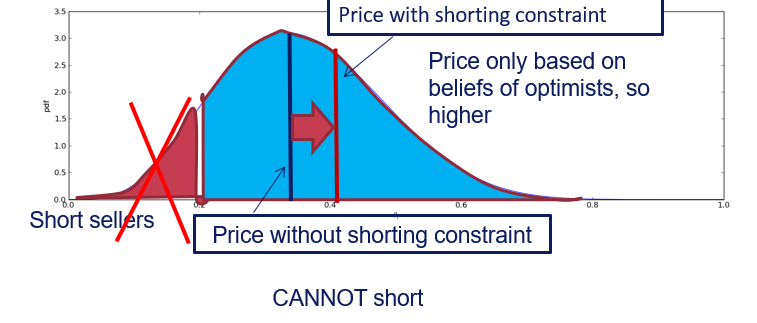
\includegraphics[width=0.55\textwidth]{figures/34.png}
\end{frame}

% --- Slide 35: Harrison and Kreps ---
\begin{frame}{Heterogeneous Beliefs with SSC, ctd.}
\begin{itemize}
\item \textbf{Dynamic argument}
\item Harrison and Kreps (1978)
\item If there are heterogeneous beliefs, you are willing to pay more than fundamental value today
  \begin{itemize}
  \item When information is released, there is a good chance that you will be the optimist
  \item You can then resell to the other agent at a higher price
  \item This creates a ``speculative'' or ``resale option'' component to the price
  \end{itemize}
\end{itemize}
\end{frame}

% --- Slide 36: Example ---
\begin{frame}{Heterogeneous Beliefs with SSC, ctd.}
\begin{itemize}
\item \textbf{An example:} $t=0,1,2$
\item Risk-neutral investors A and B trade a risky asset
\item Interest rate is zero and no short sale
\end{itemize}
\end{frame}

% --- Slide 37: Example ctd ---
\begin{frame}{Heterogeneous Beliefs with SSC, ctd.}
\begin{itemize}
\item Both agents' buy-and-hold valuation of the asset is 50
\item What is the traded price?
  \begin{itemize}
  \item In state $u$, A sets the price at 90
  \item In state $d$, B sets the price at 25
  \item Then, at time 0, both value the asset at 57.5!
  \end{itemize}
\item The price exceeds the expected value because of the resale option
\end{itemize}
\end{frame}

% --- Slide 38: Bubble Characteristics ---
\begin{frame}{Heterogeneous Beliefs with SSC, ctd.}
\begin{itemize}
\item Characteristics of this bubble component:
\item The valuation of the resale option is determined by fluctuation of agents' beliefs and asset float
\item Scheinkman and Xiong (2003): the more likely their beliefs are to diverge in the future, the larger the bubble
\item Float: More shares available for trading $\Rightarrow$ smaller bubble
\end{itemize}
\end{frame}

% --- Slide 39: High Valuations and Trading ---
\begin{frame}{Heterogeneous Beliefs with SSC, ctd.}
\begin{itemize}
\item Models of heterogeneous beliefs with SSC are popular because they not only explain overpricing, but also another important empirical fact:
\item \textbf{The coincidence of high valuations and heavy trading}
\item Evidence: Hong and Stein (2007)
\end{itemize}
\vfill
\centering
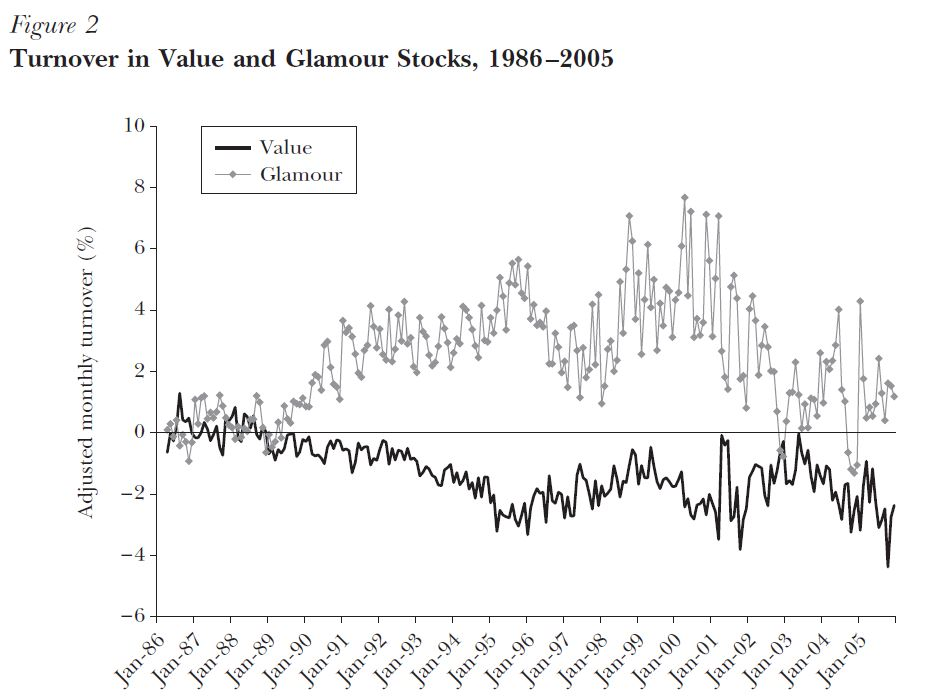
\includegraphics[width=0.40\textwidth]{figures/slide39_pic4.jpg}
\end{frame}

% --- Slide 40: Chinese Warrant Bubble ---
\begin{frame}{Heterogeneous Beliefs and Bubbles}
\begin{columns}[T]
\begin{column}{0.50\textwidth}
\begin{itemize}
\item Xiong and Yu (AER 2011) conduct a more rigorous test of the heterogeneous beliefs-based bubble theory --- The Chinese Warrant Bubble
\item In 2005--2008, over a dozen put warrants traded in China went so deep out-of-the-money that their intrinsic value was essentially zero
\item Yet they traded at high prices with enormous turnover
\end{itemize}
\end{column}
\begin{column}{0.48\textwidth}
\centering
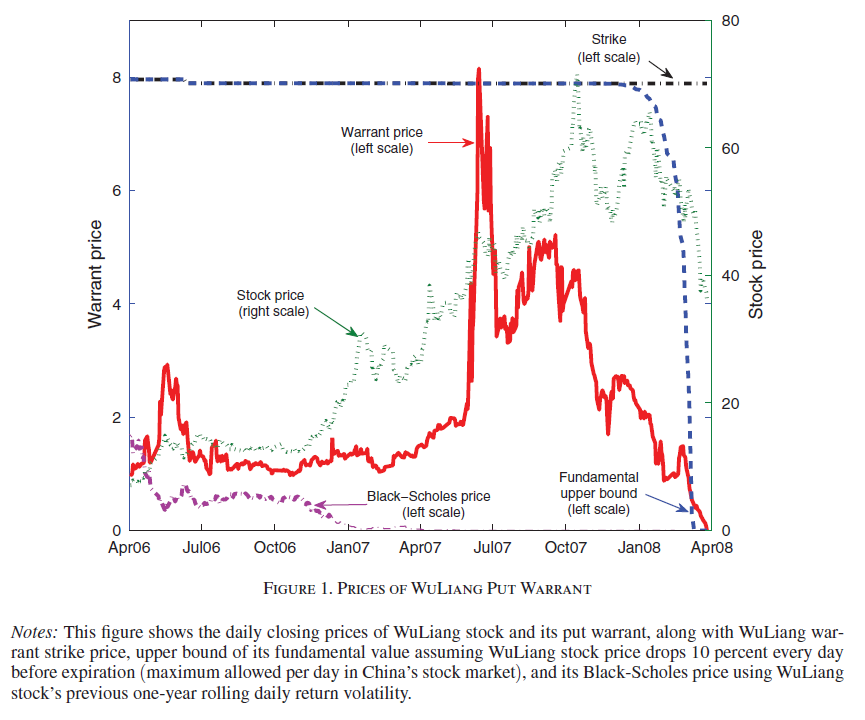
\includegraphics[width=\textwidth]{figures/slide40_pic3.png}
\end{column}
\end{columns}
\end{frame}

% --- Slide 41: Warrant Bubble Evidence ---
\begin{frame}{Heterogeneous Beliefs and Bubbles}
\begin{itemize}
\item They find evidence most consistent with resale option theory of bubble
\item The size of the warrant bubble increases with turnover and volatility, and decrease with asset float
\end{itemize}
\vfill
\centering
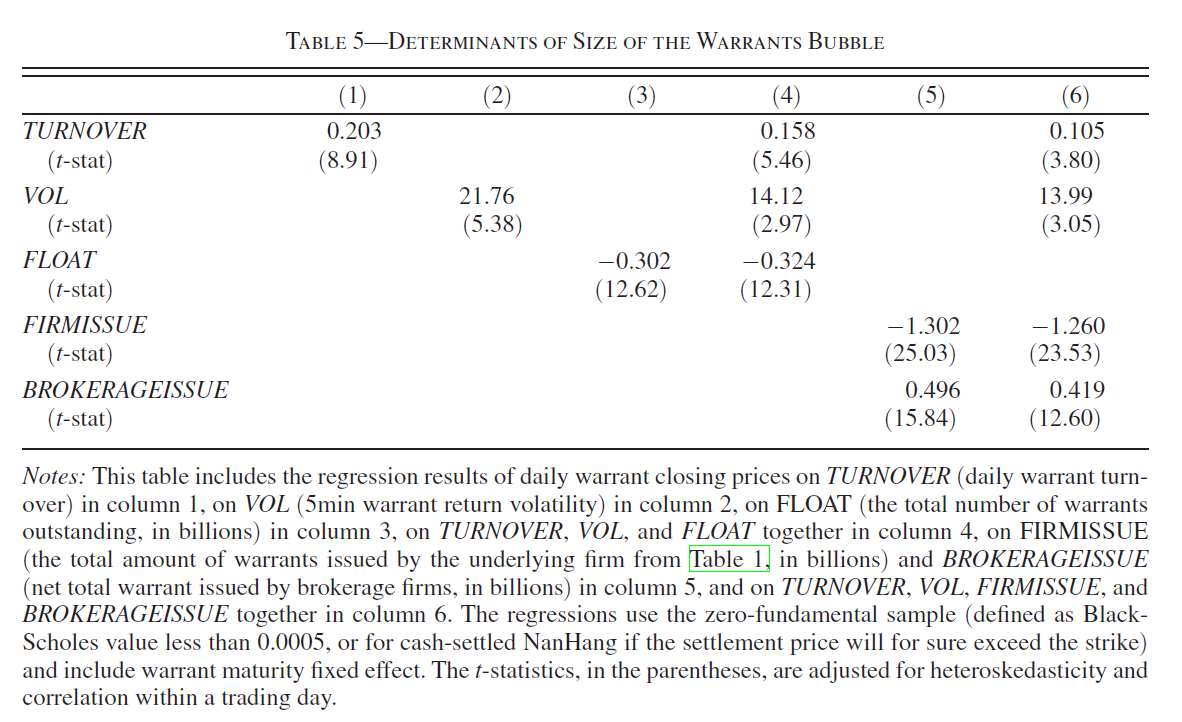
\includegraphics[width=0.55\textwidth]{figures/slide41_pic4.png}\\[0.2em]
\footnotesize Xiong and Yu (AER 2011)
\end{frame}

% --- Slide 42: Cross-Sectional Returns ---
\begin{frame}{Heterogeneous Beliefs and Cross-Sectional Stock Returns}
\begin{itemize}
\item XS prediction of models of heterogeneous beliefs with short-sale constraints:
\item Assets that people disagree about more should be more overpriced
\item Diether, Malloy, and Scherbina (JF 2003) test the model's prediction using analyst forecast dispersion as a proxy for disagreement
\item They find that stocks with higher analyst forecast dispersion earn lower future returns
\end{itemize}
\vfill
\centering
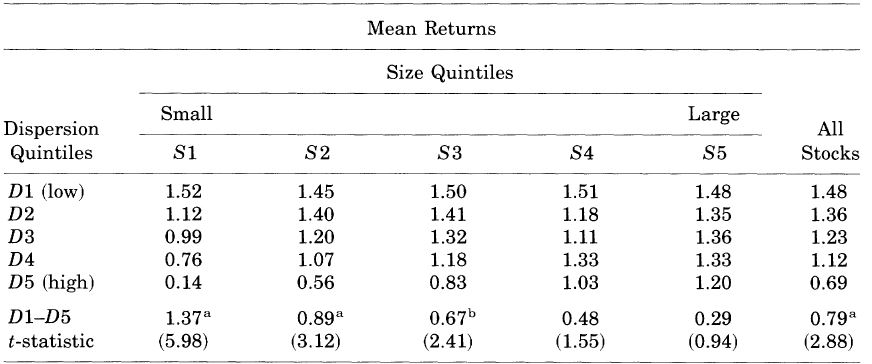
\includegraphics[width=0.50\textwidth]{figures/slide42_pic4.jpg}
\end{frame}

% --- Slide 43: Aggregate Stock Market ---
\begin{frame}{Heterogeneous Beliefs and Aggregate Stock Market}
\begin{itemize}
\item Yu (2011) tests this prediction for aggregate stock market
\item Aggregate disagreement is measured as the value-weighted average of stock-level dispersion
\end{itemize}
\vfill
\centering
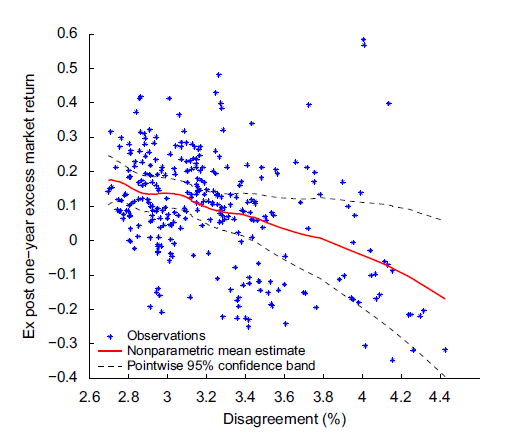
\includegraphics[width=0.45\textwidth]{figures/slide43_pic4.png}
\hspace{0.3em}

\includegraphics[width=0.45\textwidth]{figures/slide43_pic5.png}
\end{frame}

% --- Slide 44: Risk-Return Tradeoff ---
\begin{frame}{Heterogeneous Beliefs and Risk-Return Tradeoff}
\begin{itemize}
\item Another important application: risk-return tradeoff
\item Standard theory: higher risk $\Rightarrow$ higher expected return
\item But empirically, the relation between risk and return can be negative
\item Heterogeneous beliefs models can explain this anomaly
\end{itemize}
\end{frame}

% --- Slide 45: Risk-Return Tradeoff ctd ---
\begin{frame}{Heterogeneous Beliefs and Risk-Return Tradeoff}
\begin{columns}[T]
\begin{column}{0.48\textwidth}
\centering
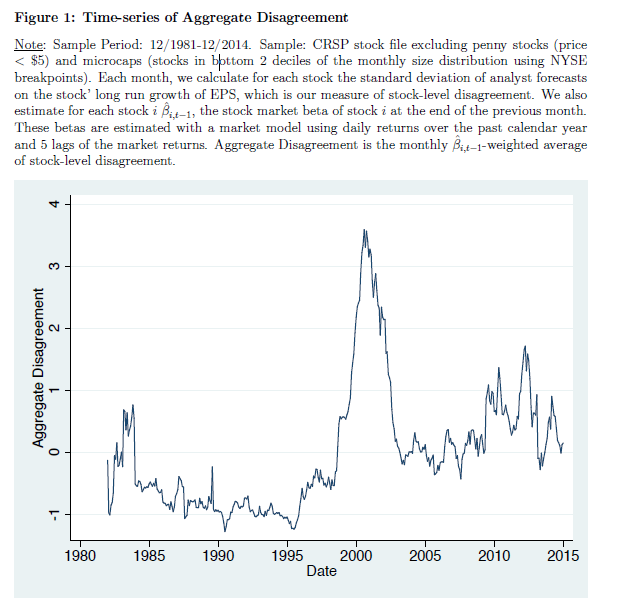
\includegraphics[width=\textwidth]{figures/slide45_pic2.png}
\end{column}
\begin{column}{0.50\textwidth}
\begin{itemize}
\item When investors disagree, the pessimists are sidelined by short-sale constraints
\item The optimists set the price
\item Higher disagreement $\Rightarrow$ higher price $\Rightarrow$ lower expected return
\end{itemize}
\end{column}
\end{columns}
\end{frame}

% --- Slide 46: Risk-Return Tradeoff ctd2 ---
\begin{frame}{Heterogeneous Beliefs and Risk-Return Tradeoff}
\vfill
\centering
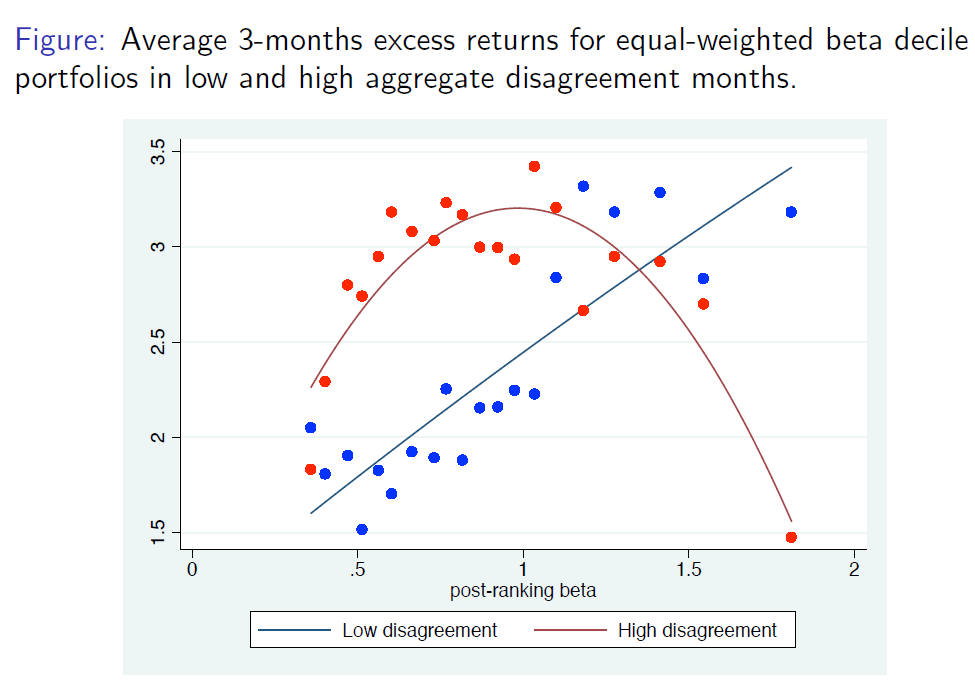
\includegraphics[width=0.45\textwidth]{figures/slide46_pic3.png}
\hspace{0.3em}
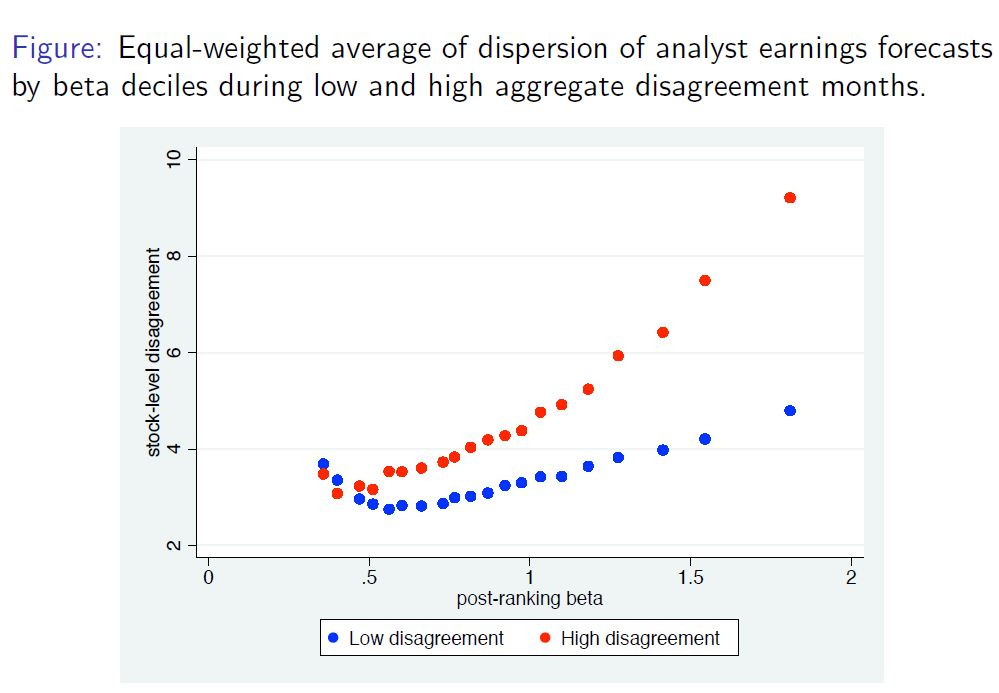
\includegraphics[width=0.45\textwidth]{figures/slide46_pic4.jpg}
\vfill
\end{frame}

% --- Slide 47: Macro Factors ---
\begin{frame}{Heterogeneous Beliefs and Risk-Return Tradeoff}
\begin{itemize}
\item The same intuition can explain the pricing of macroeconomic factors (Li 2016)
\end{itemize}
\vfill
\centering
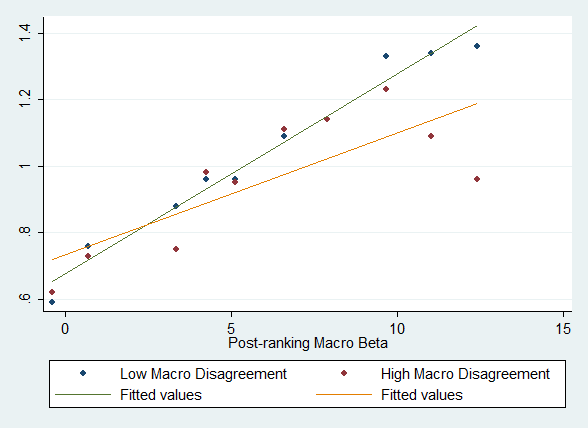
\includegraphics[width=0.55\textwidth]{figures/slide47_pic4.png}
\end{frame}

% --- Slide 48: Causal Effect ---
\begin{frame}{The Causal Effect of Disagreement on Asset Prices}
\begin{itemize}
\item Identifying exogeneous shocks to investor disagreement is still challenging
\item Chang, Hsiao, and Ljungqvist (JF 2022):
  \begin{itemize}
  \item Exploits the staggered implementation of EDGAR by SEC, which induces a reduction in information acquisition cost
  \item This leads to lower disagreement and lower stock prices
  \end{itemize}
\end{itemize}
\end{frame}

% --- Slide 49: Causal Evidence ---
\begin{frame}{The Causal Effect of Disagreement on Asset Prices}
\vfill
\centering
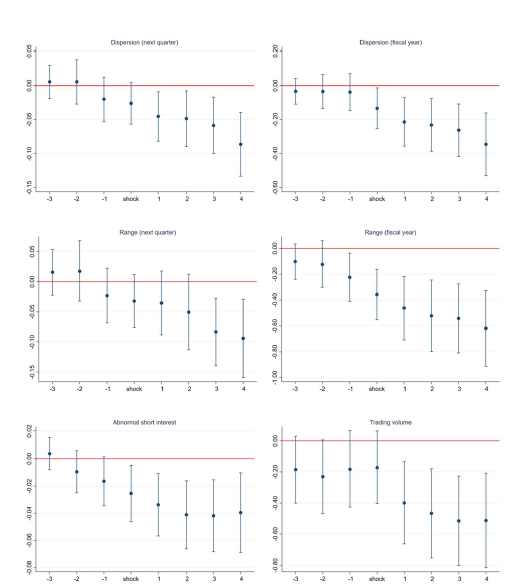
\includegraphics[width=0.30\textwidth]{figures/slide49_pic4.png}
\hspace{0.2em}
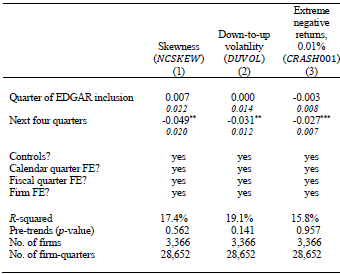
\includegraphics[width=0.30\textwidth]{figures/slide49_pic5.png}
\hspace{0.2em}
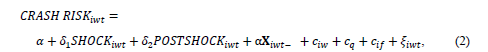
\includegraphics[width=0.30\textwidth]{figures/slide49_pic6.png}
\vfill
\end{frame}

% --- Slide 50: Concerns ---
\begin{frame}{Biased Beliefs: Concerns}
\begin{itemize}
\item Do people simply learn their way out of biased beliefs?
\item Only to a limited extent
\item Many of the most persistent behavioural biases are useful mental shortcuts for human evolution
  \begin{itemize}
  \item ``Loss aversion'' increases survival probability
  \item Overconfidence increases effort and social status
  \end{itemize}
\item Smart people can be more susceptible to some biases
  \begin{itemize}
  \item E.g.\ confirmation bias (Stanovich et al., 2013)
  \end{itemize}
\end{itemize}
\end{frame}

% --- Slide 51: Stakes ---
\begin{frame}{Stakes and Investor Biases}
\begin{itemize}
\item Sui and Wang (2025 JFE): investors do better when they care less
\item Unique setting where investors trade stocks in real accounts using their own money and simultaneously in a simulated setting
\item With lower stakes, investors trade less, diversify more, and earn higher returns
\end{itemize}
\vfill
\centering
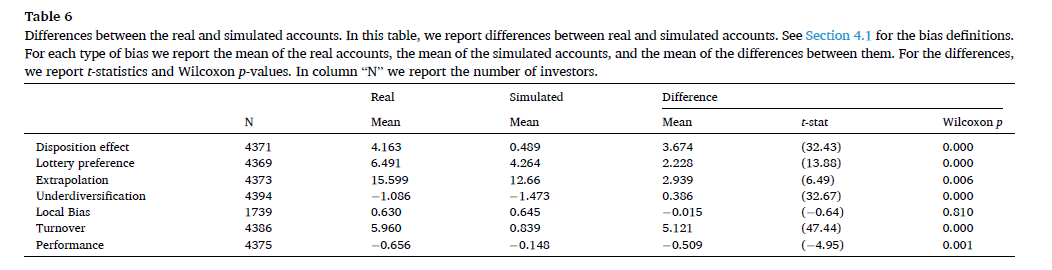
\includegraphics[width=0.70\textwidth]{figures/slide51_pic4.png}
\end{frame}

\end{document}
